%!TEX root = /Users/domaubert/Documents/Lectures/cosmologie/cosmo_main.tex
\chapter{Etat des connaissances}

%\textit{Ce chapitre est tiré de \textbf{The Cosmological Parameters}, Lahav et Liddle, arxiv1401.1389}
%\newline
%\newline

L'objectif de ce chapitre est de faire un court panorama de l'état de nos connaissances sur les propriétés observées de l'Univers. Les chapitres suivants seront eux consacrés à l'élaboration des concepts et des théories qui permettent de rendre compte de ces propriétés observées. 

Concernant notre connaissance des propriétés de l'Univers, elle repose souvent sur \textit{l'interprétation d'observations au travers de théories et de modèles}. Par conséquent les propriétés décrites dans ce chapitre sont essentiellement valables dans le contexte du modèle standard de la cosmologie\index{modèle standard} décrit dans les chapitres suivants. Si un changement de paradigme vient à opérer, rien n'empêche à priori que ces observations soit réinterprétées et donc conduisent à modifier ce que nous savons de l'Univers.

\section{Observation fondamentale : le décalage vers le rouge}
L'observation première de la cosmologie, à l'origine même de l'émergence de la discipline au début du 20ème siècle, est la constatation que tous les objets observés à grande distance sont plus "rouges" qu'attendus. La mesure du spectre\index{spectre} de ces objets indiquent que les systèmes de raies observés, parfois complexes, sont tous à des longueurs d'ondes plus importantes que ce que l'observation de ces mêmes éléments aurait donné dans un laboratoire. On définit le décalage vers le rouge ou "redshift" par la quantité z\index{redshift}
\begin{equation}
z\equiv\frac{\lambda-\lambda_0}{\lambda_0},
\end{equation}
où $\lambda$ est la longueur d'onde\index{longueur d'onde}\sidenote{avec $\lambda=cT=c/\nu$ où $T$ et $\nu$ sont respectivement les périodes\index{période!rayonnement electromagnétique} et fréquences\index{fréquence!rayonnement électromagnétique} d'oscillation de l'onde électromagnétique associée} observée et $\lambda_0$ celle mesurée en laboratoire. En corrélant cette quantité avec la distance des objets, on observe que ce rougissement est d'autant plus grand que la source est éloignée. 

Dans le cadre du modèle standard de la cosmologie, ce rougissement est de nature \textit{cosmologique} et traduit le phénomène \textit{d'expansion}\index{expansion} de l'Univers. Dans ce processus d'expansion, toute distance prise entre 2 points de l'Univers est amenée à évoluer \sidenote{en l'occurrence à augmenter dans un modèle standard d'Univers}. Notons dès à présent que cette augmentation n'est pas le symptôme d'un déplacement des sources par rapport à leur espace local mais plutôt la conséquence d'une 'dilatation' de l'espace entre l'observateur et la source. Cette dilatation agit également sur la longueur d'onde des photons\index{photon}\sidenote{et donc sur leur énergie donnée par $E=h\nu=hc/\lambda$} en vol et conduit au rougissement observé. Cette dilatation agit aussi sur les densités, diluant au cours du temps de telles quantités et on peut montrer qu'elle produit des dilatations des durées, on allongeant tout type d'intervalles temporels. Enfin, cette interprétation cosmologique permet également d'expliquer pourquoi ce décalage vers le rouge est d'autant plus important que la source est éloignée.

Notons que comme le redshift croît avec la distance, $z$ est de façon indirecte un indicateur de \textit{distance} et comme la lumière nous parvient avec une vitesse finie et connue, $z$ est également un indicateur de \textit{l'époque} à laquelle la source est observée. En cosmologie, l'action de désigner un objet ou un phénomène par son redshift $z$ implique à la fois une information spectrale, spatiale et temporelle.

Le processus d'expansion a débuté il y a 13.8 milliards d'années: c'est le \textit{Big-Bang}\index{Big-Bang}. Aux premiers instants, les distances étaient présumément courtes, l'Univers était donc de fait très dense. Régnait également une température\index{température} très élevée, qui fut amenée à décroître au cours du temps\sidenote{Par exemple la température du 'gaz de photons cosmiques', le fond diffus cosmologique, est aujourd'hui de 2.73 K mais était environ 1000 fois plus chaud lorsqu'il a été libéré il y a 380 000 ans }. De fait le modèle accepté permettant de décrire les origines de l'Univers est parfois dénommé modèle du \textit{Big Bang chaud}.

\section{Propriétés générales de l'Univers}
L'Univers dans lequel nous vivons peut, semble-t-il, être décrit par une poignée de paramètres. La connaissance de ceux-ci, ajoutée à la connaissance de ce que nous croyons être les bonnes lois de la physique, permet d'expliquer une très grande partie des propriétés globales de l'Univers et également une grande partie des processus astrophysiques qui subissent la cosmologie qui les entoure.  

\subsection{Paramètres cosmologiques\index{paramètre cosmologique}}
Comme détaillé dans les chapitres suivant, l'Univers peut être décrit à un haut niveau de précision en considérant qu'il est homogène, isotrope et possédant une dynamique régie par les équations de la relativité générale\index{relativité générale}. Toutefois cette description nécessite la connaissance à priori de certains paramètres qui permettent d'expliquer l'Univers tel qu'il est observé. L'observation de l'état actuel du cosmos met des contraintes sur la valeur de ces paramètres et nous détaillons ci-dessous les plus importants d'entre eux.

\paragraph{Paramètre de Hubble} Le premier paramètre est le paramètre de Hubble $H_0$ \index{Hubble!paramètre}, qui caractérise le taux d'expansion actuel. Sa valeur est d'environ 70 km/s/Mpc et indique qu'un objet situé à 1 Mpc\sidenote{1 Mégaparsec vaut environ $3.08\times 10^{22}$ m} s'éloignerait de nous à 70 km/s s'il était soumis uniquement à l'expansion. On utilise parfois le paramètre de Hubble réduit $h$ tel que $H_0=100 h$ km/s/Mpc~: sa valeur est proche $h\sim 0.7$.

\paragraph{Paramètres de densité} Les différents types d'énergies présentes dans l'Univers ont une grande influence sur ses propriétés et leurs contributions au budget énergétique total sont caractérisées par des paramètres de densité $\Omega_i$ \index{paramètre de densité}. En pratique, $\Omega_i$ représente le rapport de la densité d'énergie de type $i$ à une densité d'énergie de référence appelée \textit{densité critique\index{densité critique}}. On distingue la densité de matière $\Omega_m$, la densité de baryons\index{baryon} (protons+neutrons(+électrons))\sidenote{en termes rapides, les baryons constituent la matière 'normale' à laquelle nous sommes habitués} $\Omega_b$, la densité de rayonnement $\Omega_r$, la densité d'énergie des neutrinos $\Omega_\nu$ et la densité d'énergie noire\index{energie noire@énergie noire} $\Omega_\Lambda$. Il faut noter que la contribution de la matière contient celle des baryons\index{baryon}, par conséquent $\Omega_m\ge\Omega_b$: actuellement on a $\Omega_m\sim 0.3$ et $\Omega_b\sim 0.05$, la différence étant la contribution apportée par une matière \textit{non baryonique} et invisible, appelée la matière noire\index{matière noire}. Les contributions des espèces relativistes (photons, neutrinos) est aujourd'hui négligeable, bien que ce type de particules soit très abondant en nombre.

\paragraph{Spectre de fluctuations initiales} L'Univers tel qu'observé actuellement n'est pas strictement homogène, en particulier sur des échelles inférieures à la dizaine de Mpc. Les galaxies et amas qui nous entourent trouvent leur origine dans des fluctuations\index{fluctuations de densité} initiales de densité de très faible amplitude. Ces fluctuations sont caractérisées par un spectre dit 'de puissance'  $P(k)$\index{spectre de puissance} qui donne la distribution des amplitudes des fluctuations de taille $L=2\pi/k$. On suppose actuellement que celles-ci trouvent leur origine dans la période \textit{d'Inflation}\index{Inflation} qui prédit un spectre primordial de la forme \index{spectre de puissance} 
\begin{equation}
P(k)\sim  k^{n_s}.
\end{equation} 
$n_s$ constitue également un paramètre cosmologique et les modèles Inflationnaire lui prédise une valeur \textit{proche mais différente} de l'unité \sidenote{le satellite Planck mesure ainsi une valeur proche de 0.96}. L'amplitude globale du spectre doit également être paramétrée, par exemple sous la forme d'une amplitude de fluctuation sur une échelle arbitraire de 8 Mpc, notée $\sigma_8$\index{spectre de puissance! amplitude}. Notons enfin que les modèles d'Inflation prédisent un fond d'ondes gravitationnelles\index{ondes gravitationnelles}, caractérisé par un spectre de fluctuations tensorielles, similaire à celui des fluctuations de densité (dites également scalaires). Le rapport d'amplitude entre fluctuations tensorielles et scalaires est noté $r$ et sa valeur est supposée faible.

\paragraph{Etat d'ionisation de l'Univers} Le dernier paramètre canonique de la cosmologie permet de décrire l'état d'ionisation \index{ionisation} de l'Univers au cours de son histoire. Cet état se mesure en  contraignant le nombre moyen de diffusions des photons\index{photon} sur les électrons libres du cosmos\index{electron@électron}. Cette quantité est notée $\tau$ avec une valeur typique $\tau \sim 0.07$. L'essentiel de ces électrons libres sont produits au cours de la Réionisation \index{Réionisation} de l'Univers au redshift $z_\mathrm{reion}\sim 8-6$\sidenote{environ 1 milliard d'années après le Big-Bang}: dans les modèles les plus simples $\tau$ et $z_\mathrm{reion}$ sont directement liés.

\paragraph{Modèle minimal} L'ensemble des paramètres décrits précédemment permet de rendre compte d'une grande variété de propriétés observables. D'autre part, certaines hypothèses permettent encore de réduire le nombre de paramètres libres. Par exemple, l'Inflation prédit une courbure\index{courbure} intrinsèque nulle qui se traduit en pratique par $\sum_i \Omega_i=1$. D'autre part l'amplitude des modes tensoriels (i.e. les ondes gravitationnelles issues de l'Inflation) étant attendue comme très faible, on peut aisément poser $r=0$. Enfin, le paramètre de densité de rayonnement $\Omega_r$ est très précisément connue, par la mesure précise de la température  du fond diffus\index{fond diffus cosmologique} ($T=2.7255\pm0.0006$ K) et ne permet donc plus de latitude significative sur sa valeur. Enfin , en l'absence de physique exotique la densité d'énergie des neutrinos $\Omega_\nu$ est directement liée à celle des photons \sidenote{tout en étant quasi nulle aujourd'hui}. Au final, un modèle extrêmement solide peut être construit avec seulement 6 paramètres libres. Un choix typique de "sextet" est $(\Omega_b,\Omega_m, H_0,\sigma_8,n_s,\tau)$. Bien sûr d'autres combinaisons de paramètres libres sont possibles.

\subsection{Principales sondes observationnelles}

Les paramètres précédents sont contraints par l'observation croisée de différentes sondes observationnelles. La convergence de ces valeurs conduit à ce qui est communément nommé \textit{le modèle de concordance} ou \textit{modèle standard}\index{modèle standard}. Voici une liste (non-exhaustive) de ces sondes cosmologiques.

\paragraph{Mesure directe de $H_0$}
Cette mesure s'effectue à l'aide de chandelles standards qui permettent de mesurer indépendamment la distance d'un objet extra-galactique et son redshift $z$. La chandelle de référence est la relation période-luminosité des étoiles variables de type Céphéides\index{Céphéides} : la mesure de la période de variation de leur flux apparent permet de déterminer leur luminosité intrinsèque \sidenote{une Céphéide intrinsèquement brillante varie lentement, une Céphéide faible varie rapidement} et la connaissance de ce flux et cette luminosité permet d'obtenir la distance\sidenote{via $\mathrm{Flux}=\mathrm{Lum}/4\pi (\mathrm{dist})^2$ }. Les Céphéides sont des indicateurs primaires et permettent de calibrer des indicateurs secondaires: courbes de lumières des supernovæ, relation de Tully-Fisher\sidenote{qui relie la luminosité d'une galaxie à sa vitesse de rotation}, etc... Ce type d'indicateurs donne une valeur de $H_0\sim 73$ km/s/Mpc. Le fond diffus cosmologique permet également une mesure indépendante de $H_0\sim 67$ km/s/Mpc en légère tension avec les estimateurs précédents.

\paragraph{Supernovæ\index{supernovae} et cosmologie}
La grande luminosité des supernovæ permet leur détection à des distances cosmologiques : ce terme désigne les stades finaux des étoiles les plus massives incapables de maintenir des réactions de fusion nucléaires en leur sein, conduisant à leur explosion. De plus certains types de supernovæ\index{supernovae}, celles dite de type 'SN1A', ont un caractère quasi standard car elles résultent de l'explosions de naine blanche dans des systèmes binaires pour lesquelles il existe une forte corrélation entre luminosité et paramètres de la courbe de luminosité\index{courbe de luminosité}. L'accélération\index{accélération!expansion} \sidenote{c'est-à-dire le fait que les distances augmentent de plus en plus rapidement aujourd'hui} de l'expansion de l'Univers a été mise en évidence pour la première fois à l'aide de ce type d'indicateurs, en proposant pour la première fois la combinaison $\Omega_m\sim0.3$ et $\Omega_\Lambda\sim0.7$. De plus ces mêmes indicateurs indiquent que la densité d'énergie noire\index{energie noire@énergie noire} est probablement une constante en temps et en espace, donc équivalente à une constante cosmologique\index{constante cosmologique}\sidenote{on rencontrera aussi parfois le terme d'énergie du vide}.

\paragraph{Le fond diffus cosmologique}
Le fond diffus\index{fond diffus cosmologique} cosmologique (Cosmic Microwave Background, CMB) est constitué des photons produits lors de la Recombinaison\index{Recombinaison}, 380 000 ans après le Big-Bang. Il constitue le plus grand réservoir de photons\index{photon} du cosmos et présente une brillance homogène à des niveaux de 1 pour 100 000. En deçà de ces niveaux, le CMB présente néanmoins de faibles inhomogénéités qui tracent les inhomogénéités de matière à cette époque. Leur structure spatiale (en fait angulaire sur le ciel) comprend des informations sur toute l'histoire de croissance des structures depuis le Big-Bang jusqu'à 380 000 ans plus tard et sur les processus de couplage entre le rayonnement et la matière. L'étude de ces fluctuations permet par exemple d'établir la platitude de la géométrie de l'Univers\index{géométrie de l'Univers}, fournit une mesure de la quantité de baryons $\Omega_b$\index{baryon}, confirme la nécessité d'une matière non-baryonique\index{matière noire} et l'absence d'évolution de l'énergie noire. Le CMB indique également que le spectre de fluctuation initial\index{spectre de puissance} est compatible avec les modèles d'Inflation \index{Inflation} et pour l'instant les modes tensoriels restent indétectables. Enfin le nombre de diffusions \index{photon!diffusion} des photons sur les électrons est de l'ordre de $\tau\sim 0.07$ correspondant à une Réionization vers un redshift de $z\sim8$. Le CMB constitue à l'heure actuelle la sonde la plus précise et la plus complète d'informations cosmologiques. C'est l'objet d'étude de missions spatiales et sol de très grande ampleur, dont par exemple le satellite européen \textit{Planck}.

\begin{figure}[htbp]
	\centering
		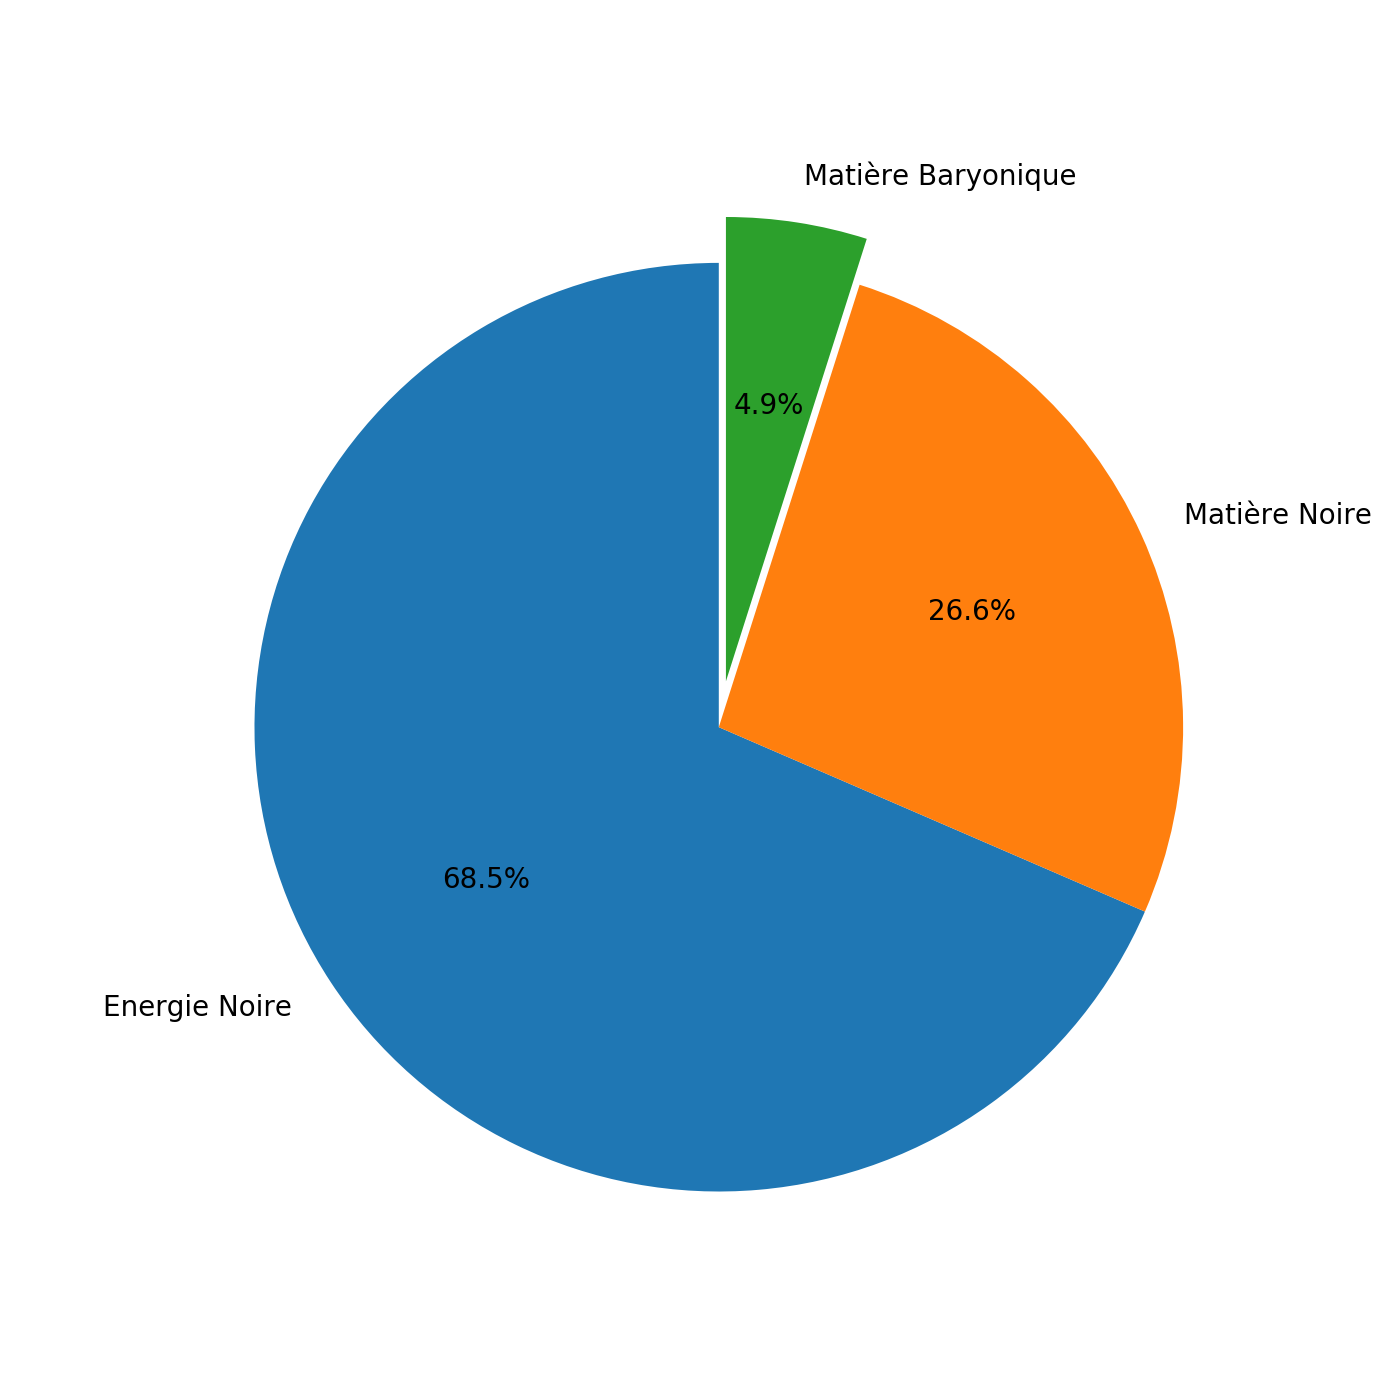
\includegraphics[height=10cm]{figs/pieplanck.png}
		\caption[Le bilan énergétique de l'Univers]{La répartition des différentes formes d'énergie au bilan énergétique total de l'Univers, d'après les mesures du satellite \textit{Planck}. On note l'absence de contribution du rayonnement et des neutrinos, dont le poids énergétique est trop faible pour pouvoir être représenté ici. La matière 'normale', désignée comme 'baryonique' et composée de protons, neutrons et électrons ne représente que $\sim 5\%$ du total. Le reste constitue le \textit{secteur sombre}.}
	\label{f:timeline}
\end{figure}


\paragraph{Grands relevés de Galaxies}
Les galaxies \index{galaxie} constituent des traceurs (biaisés) de la distribution de matière dans le cosmos. Par conséquent des efforts importants sont réalisés pour collecter de façon homogène, les positions dans le ciel et les propriétés de millions de galaxies, sous forme de grands relevés : parmi les plus connus on citera le \textit{Sloane Digital Sky Survey}, SDSS, ou bien le futur relevé du satellite européen \textit{Euclid}\sidenote{prévu pour voler en 2021}. En théorie, l'étude de la distribution spatiale de ces objets dans des grands relevés\index{grands relevés} doit permettre de contraindre le déroulé du processus de croissance des structures de l'Univers\index{grande structure de l'Univers} et par extension la cosmologie. Parmi les mesures les plus spectaculaires autorisées par ce type de relevés est la détection des oscillations baryoniques acoustiques\index{oscillation baryonique acoustique} (BAOs) à bas redshift. Les BAOs sont déclenchés dans l'Univers pré-Recombinaison et consistent en des ondes acoustiques dans le gaz baryonique entretenues par la compétition entre la pression de rayonnement et la gravitation produite par toute la matière. Ces BAOs sont gelés après la Recombinaison\index{Recombinaison} et se manifestent sur des échelles d'environ 150 Mpc dans toute distribution de matière qui échantillonnent ces distances, dont le CMB et les grands relevés de galaxies.  La cosmologie issue des relevés de galaxies permet généralement de lever les dégénérescences entre paramètres\sidenote{on parle de dégénérescences quand plusieurs combinaisons de paramètres permettent de reproduire une même observation. Impossible alors de distinguer laquelle est la meilleure.}, par exemple pour les estimations issues du CMB, et sont donc d'une importance essentielle. De plus les relevés opèrent à différents redshifts $z$ et offrent  des vues à différents instants d'une même sonde cosmologique (par exemple sur les BAOs) et sont donc des outils extrêmement puissants.

\paragraph{Amas de Galaxies}
Les amas de galaxies\index{amas de galaxies} constituent les plus grands objets qui se sont effondrés gravitationnellement aujourd'hui. Ils peuvent comprendre plusieurs milliers de galaxies et atteindre des masses allant jusqu'à $10^{15} M_\odot$. Le décompte de ces objets et leur fonction de masse permet ainsi de contraindre le champ de matière aux échelles qui viennent seulement de s'effondrer, sous l'action de la gravité\sidenote{on parle aussi de passage au régime non linéaire pour l'effondrement, en référence à la nature non linéaire des équations qui permettent de décrire ce processus}. Généralement on extrait de l'étude des amas les quantités $\sigma_8\sim 0.8$ et $\Omega_m\sim0.3$. Ces amas sont généralement des émetteurs X, dont l'émissivité permet de déterminer la masse. On les détecte également dans le signal du CMB comme des distorsions locales du spectre via l'effet Sunyaev-Zeldovich\index{Effet Sunyaev-Zeldovich}.

\paragraph{Milieu Intergalactique}
La structure du gaz dans le milieu intergalactique\index{milieu intergalactique} (IGM) nous renseigne également sur la distribution spatiale de la matière à différents redshifts, via la mesure du spectre de puissance\index{spectre de puissance} de la matière $P(k)$. La sonde la plus commune de l'IGM est la \textit{forêt Lyman-alpha}\index{forêt Lyman-$\alpha$}, qui se manifeste dans les spectres de quasars distants comme un ensemble de raies d'absorptions qui tracent la distribution de nuages absorbants le long de la ligne de visée. Dans le meilleur de cas, les BAOs\index{BAO} peuvent même être retrouvés (c'est le cas par exemple vers $z\sim2$) grâce à de multiples spectres pris le long de multiples directions vers des quasars\index{quasar} différents. Une autre application de l'étude de l'IGM pour la cosmologie consiste à observer les tunnels d'absorptions dans les spectres de quasars à très grand redshift $z>5.5$ : l'Univers y est jeune ($t<1$ Gyr) et encore neutre. La mesure de ces tunnels permet de contraindre l'histoire de la Réionisation\index{Réionisation} de l'Univers et le paramètre cosmologique $\tau$.

\paragraph{Lentilles Gravitationnelles}
Les lentilles gravitationnelles\index{lentille gravitationnelle} traduisent la déformation de l'espace temps à proximité d'objets massifs, ce qui conduit également à une déformation de la trajectoire des rayons lumineux entre une source et un observateur. Dans les cas les plus spectaculaires(lentillage fort ou \textit{strong lensing}) à proximité d'amas de galaxies  cela conduit à la production d'images multiples et à de fortes déformations de types arcs gravitationnels. Sur de grandes portions du ciel, le signal est beaucoup plus modéré bien que l'on s'attende à ce que par exemple le CMB ou bien la distribution de galaxies à un certain $z$ soient déformés par la distribution de matière entre eux et nous observateurs (lentillage faible ou \textit{weak lensing}). Ces faibles déformations peuvent toutefois être analysées statistiquement pour conduire à des contraintes sur la distribution de la matière déformante via $P(k)$ et à l'amplitude des fluctuations associées $\sigma_8$.

\section{Une Histoire du Cosmos}
\begin{figure}[htbp]
	\centering
		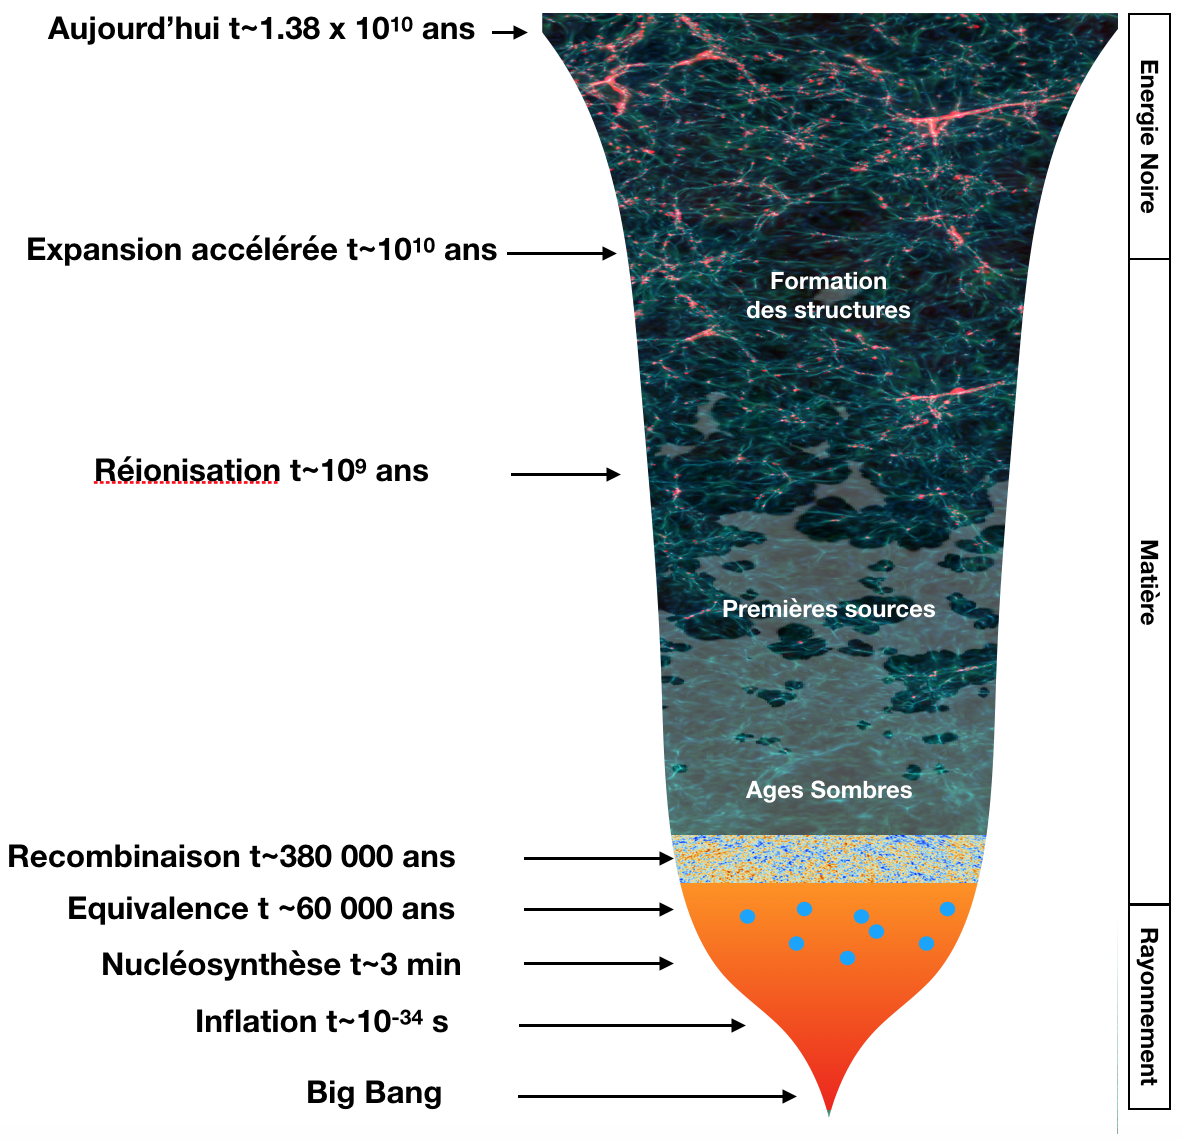
\includegraphics[height=10cm]{figs/timeline.png}
		\caption[Les grandes étapes dans l'histoire du cosmos]{Les grandes étapes dans l'histoire du cosmos. Cette frise couvre environ 13.8 milliards d'années d'évolution depuis le Big-Bang  jusqu'à nos jours. Notons que l'échelle temporelle n'est pas régulière et l'extension latérale décrit l'histoire d'évolution des distances dans le cosmos. Les grandes étapes de domination sont également indiquées. Les temps correspondent à une cosmologie standard $\Lambda CDM$.}
	\label{f:timeline}
\end{figure}

\newthought{Pour finir}, nous allons donner un court descriptif des grandes étapes de l'histoire de l'Univers. Ces grandes étapes décrivent des processus physiques ou des transitions spécifiques qui opèrent à certains stades de l'évolution du cosmos : par extension leurs noms sont aussi utilisés pour désigner des instants. Par exemple on parle de la Réionisation pour désigner la fin du premier milliard d'années de l'Univers ou bien de l'Inflation pour désigner ses premiers instants.

L'Univers a connu une phase extrêmement dense et chaude, il y a 13.8 milliards d'années. Nos théories actuelles ne nous permettent pas actuellement de remonter en deçà d'un temps de Planck ($\sim 10^{-44}$ s)\index{temps de Planck},  désignant une durée sur laquelle les effets de gravité quantique pourraient se manifester \sidenote{gravité quantique pour laquelle nous n'avons à ce jour pas de théorie satisfaisante}. A cette incertitude près, l'histoire de l'Univers débute à cette époque, nommée le \textit{Big-Bang} \index{Big-Bang}. A partir de cet instant, l'Univers va subir un effet d'expansion de l'espace et de baisse de sa température\index{température}. Dans le cadre du modèle cosmologique standard\index{modèle standard}, les grandes étapes de son évolution sont les suivantes (cf. figure \ref{f:timeline}):
\begin{enumerate}
\item \underline{L'Inflation} $t\sim 10^{-34}$ secondes\index{Inflation} :  cette phase est encore spéculative et consisterait en une phase d'expansion accélérée de l'Univers dans ces instants quasi-initiaux. Si ce processus a bien eu lieu, il permettrait d'expliquer naturellement la grande homogénéité initiale de l'Univers, sa platitude et donnerait une origine quantique aux fluctuations initiales de matière qui sont à l'origine des grandes structures\index{grande structure de l'Univers} actuelles de l'Univers. Ce processus aurait également été la source d'ondes gravitationnelles\index{onde gravitationnelle} qui seraient toujours détectables et dont la découverte signerait la confirmation de l'existence d'une phase d'Inflation.
\item \underline{l'Univers primordial} $t<3$ minutes : au cours de cette époque l'Univers reste extrêmement chaud et dense. Il s'y déroule des processus à très haute énergie: plasma quark-gluons, confinement des quarks\index{quark}, baryogénèse\index{baryogénèse} (i.e. l'annihilation matière anti-matière), découplage des neutrinos\index{neutrino}, nucléosynthèse\index{nucléosynthèse} des éléments légers jusqu'à l'hélium\index{hélium}.
\item \underline{l'Equivalence} $z=3100$ t=60 000 ans \index{equivalence@équivalence matière-rayonnement} l'Univers voit son bilan énergétique passer d'une domination par les espèces relativistes (le rayonnement) à une domination par la matière.
\item \underline{La Recombinaison}\index{Recombinaison} $z=1100$ t=380 000 ans : l'Univers devient suffisamment froid (T=3000 K) et peu dense pour permettre la création d'atomes neutres et l'émission du fond diffus\index{fond diffus cosmologique} cosmologique (CMB). 
\item \underline{les âges sombres} $1100>z>30$ \index{ages sombres@âges sombres} l'Univers est rempli de gaz froid et neutre. Le gaz se structure sous l'effet de la gravitation mais  n'est pas encore en mesure de former des étoiles\index{etoiles@étoiles}. 
\item \underline{la Réionisation} $30>z>6$ le gaz parvient à des densité lui permettant de se convertir en étoiles. Ces étoiles vont émettre un rayonnement ionisant\index{ionisation} qui vont réioniser (avec une fraction d'atomes neutres $x_\mathrm{HI}\sim0.0001$) et réchauffer totalement l'Univers ($T\sim 10000$). C'est les stades initiaux de la formation des galaxies\index{formation des galaxies}.
\item \underline{la formation des galaxies et des grandes structures} $30>z>0$ à partir de la formation des première étoiles vont se former dans les premières galaxies. Elles vont croître de façon hiérarchique \index{formation hiérarchique} par assemblage de petits objets pour former les plus gros, sous l'effet de processus d'instabilité gravitationnelle\index{instabilité gravitationnelle} dominés par une matière non baryonique. Les amas de galaxies\index{amas de galaxies} vont apparaître vers $z=1$.
\item \underline{Accélération de l'expansion cosmique}\index{expansion!accélération} $z\sim 0.3$, $t\sim 10$ milliards d'années. Le bilan énergétique de l'Univers devient dominé par l'énergie noire\index{energie noire@énergie noire}, induisant une expansion accélérée de l'Univers.
\item \underline{Aujourd'hui} $z=0$. L'Univers a 13.8 milliards d'années \index{age de l'Univers@âge de l'Univers}.
\end{enumerate}


